\documentclass[12pt,a4paper]{article}

% ─── Page Layout ───────────────────────────────────────────────────────────────
\usepackage[a4paper, margin=0.8in, headheight=14pt]{geometry}

% ─── Fonts (XeLaTeX) ───────────────────────────────────────────────────────────
\usepackage{fontspec}
\usepackage{unicode-math}
\setmainfont{TeX Gyre Pagella}
\setmonofont[Scale=0.88]{TeX Gyre Cursor}
\setmathfont{Latin Modern Math}

% ─── Packages ──────────────────────────────────────────────────────────────────
\usepackage{xcolor}
\usepackage{colortbl}
\usepackage{titlesec}
\usepackage{enumitem}
\usepackage{tabularx}
\usepackage{booktabs}
\usepackage{array}
\usepackage{amsmath}
\usepackage{tikz}
\usetikzlibrary{shapes.geometric, arrows.meta, positioning, calc, fit, decorations.pathreplacing, patterns}
\usepackage{tcolorbox}
\tcbuselibrary{skins, breakable}
\usepackage{hyperref}
\usepackage{fancyhdr}
\usepackage{graphicx}
\usepackage{microtype}
\hyphenpenalty=10000
\exhyphenpenalty=10000
\sloppy
\usepackage{caption}
\usepackage{setspace}
\usepackage{multirow}
\usepackage{tocloft}

% ─── Q&A helper ────────────────────────────────────────────────────────────────
\newcommand{\Q}[1]{\textbf{#1}\par\noindent\ignorespaces}

% ─── Colour Palette ────────────────────────────────────────────────────────────
\definecolor{myred}{RGB}{196,30,58}
\definecolor{mydark}{RGB}{30,30,50}
\definecolor{mygreen}{RGB}{14,120,80}
\definecolor{myteal}{RGB}{0,130,140}
\definecolor{myamber}{RGB}{180,100,0}
\definecolor{mypurple}{RGB}{100,30,160}
\definecolor{mygray}{RGB}{246,247,249}
\definecolor{mgframe}{RGB}{180,185,200}
\definecolor{watermark}{RGB}{145,150,170}
\definecolor{hdrred}{RGB}{250,232,235}
\definecolor{hdrgreen}{RGB}{220,244,233}
\definecolor{hdrteal}{RGB}{220,242,244}
\definecolor{hdramber}{RGB}{253,242,215}
\definecolor{hdrpurple}{RGB}{238,228,255}
\definecolor{hdrgray}{RGB}{238,240,245}
\definecolor{rowalt}{RGB}{250,251,253}

% ─── Section Formatting ────────────────────────────────────────────────────────
\titleformat{\section}
  {\large\bfseries\color{myred}}{\thesection.}{0.5em}{}
  [\vspace{1pt}{\color{myred}\rule{\linewidth}{0.8pt}}]
\titleformat{\subsection}
  {\normalsize\bfseries\color{myteal}}{\thesubsection}{0.5em}{}
\titlespacing*{\section}{0pt}{18pt}{7pt}
\titlespacing*{\subsection}{0pt}{11pt}{4pt}

% ─── Paragraph ─────────────────────────────────────────────────────────────────
\setlength{\parindent}{0pt}
\setlength{\parskip}{4pt}

% ─── TOC Styling ───────────────────────────────────────────────────────────────
\renewcommand{\cfttoctitlefont}{\large\bfseries\color{myred}}
\renewcommand{\cftaftertoctitle}{\par\noindent{\color{myred}\rule{\linewidth}{0.8pt}}}
\setlength{\cftbeforetoctitleskip}{0pt}
\setlength{\cftaftertoctitleskip}{6pt}
\renewcommand{\cftsecfont}{\normalsize\bfseries\color{mydark}}
\renewcommand{\cftsecpagefont}{\normalsize\bfseries\color{mydark}}
\renewcommand{\cftsecleader}{\cftdotfill{\cftdotsep}}
\setlength{\cftbeforesecskip}{7pt}
\renewcommand{\cftsubsecfont}{\small\color{mydark}}
\renewcommand{\cftsubsecpagefont}{\small\color{mydark}}
\setlength{\cftbeforesubsecskip}{3pt}
\setlength{\cftsubsecindent}{1.4em}

% ─── Table helpers ─────────────────────────────────────────────────────────────
\renewcommand{\arraystretch}{1.45}
\setlength{\tabcolsep}{6pt}
\arrayrulecolor{mydark}
\newcolumntype{B}[1]{>{\small\bfseries\raggedright\arraybackslash}m{#1}}
\newcolumntype{Y}{>{\small\raggedright\arraybackslash}X}
\renewcommand{\tabularxcolumn}[1]{m{#1}}

% ─── Header / Footer ───────────────────────────────────────────────────────────
\pagestyle{fancy}
\fancyhf{}
\fancyhead[L]{\small\color{myred}\textbf{BS-M301}\;\color{mydark}--- Probability and Statistics}
\fancyhead[R]{\small\color{myteal}\textbf{Module 4 Notes}}
\fancyfoot[C]{\small\color{mydark}\thepage}
\fancyfoot[R]{\small\color{watermark}\textit{\copyright\ Biraj}}
\renewcommand{\headrulewidth}{0.5pt}
\renewcommand{\footrulewidth}{0.3pt}

% ─── Hyperref ──────────────────────────────────────────────────────────────────
\hypersetup{
  colorlinks=true, linkcolor=myteal, urlcolor=myteal,
  pdfauthor={Biraj Sarkar (CGEC)},
  pdftitle={BS-M301 --- Module 4 Notes: Basic Statistics, Moments, Distributions, Correlation and Regression}
}

% ─── tcolorbox styles ──────────────────────────────────────────────────────────
\tcbset{
  tikzbox/.style={
    colback=mygray, colframe=mgframe, boxrule=0.6pt, arc=4pt,
    left=8pt, right=8pt, top=6pt, bottom=6pt,
    colbacktitle=mgframe, coltitle=mydark,
    fonttitle=\small\bfseries
  },
  defbox/.style={
    colback=hdrgreen, colframe=mygreen, boxrule=0.8pt, arc=4pt,
    left=9pt, right=9pt, top=6pt, bottom=6pt,
    colbacktitle=mygreen, coltitle=white,
    fonttitle=\small\bfseries
  },
  formulabox/.style={
    colback=hdrteal, colframe=myteal, boxrule=0.8pt, arc=4pt,
    left=9pt, right=9pt, top=7pt, bottom=7pt,
    colbacktitle=myteal, coltitle=white,
    fonttitle=\small\bfseries
  },
  examplebox/.style={
    colback=hdramber, colframe=myamber, boxrule=0.8pt, arc=4pt,
    left=9pt, right=9pt, top=6pt, bottom=6pt,
    colbacktitle=myamber, coltitle=white,
    fonttitle=\small\bfseries
  },
  masonbox/.style={
    colback=hdrpurple, colframe=mypurple, boxrule=0.8pt, arc=4pt,
    left=9pt, right=9pt, top=6pt, bottom=6pt,
    colbacktitle=mypurple, coltitle=white,
    fonttitle=\small\bfseries
  },
  exambox/.style={
    colback=hdrpurple, colframe=mypurple, boxrule=1pt, arc=5pt,
    left=10pt, right=10pt, top=8pt, bottom=8pt,
    colbacktitle=mypurple, coltitle=white,
    fonttitle=\bfseries,
    breakable, title after break={\textbf{Frequently Asked / Viva Questions (contd.)}}
  }
}
\tcbset{breakable}
\tcbset{after={\color{black}}}

% ─── TikZ styles ───────────────────────────────────────────────────────────────
\tikzset{
  arrow/.style={-Stealth, thick, color=mydark},
  redarrow/.style={-Stealth, thick, color=myred},
  line/.style={thick, color=mydark}
}

\begin{document}

% ─── Title Page ───────────────────────────────────────────────────────────────
\begin{center}
  {\LARGE\bfseries\color{myred} BS-M301 --- Probability and Statistics}\\[5pt]
  {\normalsize\color{mydark} Semester III \quad$\bullet$\quad 3L:0T:3P \quad$\bullet$\quad 3 Credits}\\[3pt]
  {\normalsize\color{myteal}\textbf{Module 4 Exam Notes: Basic Statistics, Moments, Distributions, Correlation and Regression}}\\[3pt]
  {\small\color{mydark} CGEC \;$|$\; B.Tech ECE (2023--27) \;$|$\; \textit{Biraj Sarkar}}
\end{center}
\vspace{2pt}
\noindent{\color{myred}\rule{\linewidth}{1.5pt}}
\vspace{2pt}

\hypersetup{linkcolor=mydark}
\tableofcontents
\hypersetup{linkcolor=myteal}
\newpage

% ───────────────────────────────────────────────────────────────────────────────
\section{Measures of Central Tendency, Moments, Skewness and Kurtosis}
% ───────────────────────────────────────────────────────────────────────────────

Descriptive statistics provides quantitative summaries describing the central clustering, dispersion, asymmetry, and peakedness of experimental datasets.

\begin{tcolorbox}[defbox, title={\textbf{Definition: Measures of Central Tendency}}]
\begin{enumerate}[leftmargin=*, itemsep=2pt, topsep=2pt]
  \item \textbf{Arithmetic Mean ($\bar{x}$):} The sum of all observations divided by sample size:
  \begin{equation}
    \bar{x} = \frac{1}{N} \sum_{i=1}^n f_i x_i, \qquad N = \sum_{i=1}^n f_i
  \end{equation}
  \textit{Key Properties:} (1) Algebraic sum of deviations is zero: $\sum f_i (x_i - \bar{x}) = 0$. (2) Sum of squared deviations is minimal about the mean: $\sum f_i (x_i - A)^2$ is minimum when $A = \bar{x}$.
  \item \textbf{Median ($M$):} The middle value partitioning the ordered dataset into two equal halves. For grouped data with median class $[L, L+h]$:
  \begin{equation}
    M = L + \frac{\frac{N}{2} - C}{f} \cdot h
  \end{equation}
  where $L$ is lower boundary, $C$ is cumulative frequency of preceding class, and $f$ is frequency.
  \item \textbf{Mode ($Z$):} The most frequently occurring value in the distribution:
  \begin{equation}
    Z = L + \frac{f_1 - f_0}{2f_1 - f_0 - f_2} \cdot h
  \end{equation}
  \textbf{Empirical Relationship for Moderately Skewed Distributions:}
  \begin{equation}
    \text{Mode} \approx 3 \times \text{Median} - 2 \times \text{Mean} \iff \text{Mean} - \text{Mode} \approx 3(\text{Mean} - \text{Median})
  \end{equation}
\end{enumerate}
\end{tcolorbox}

\subsection{Moments and Moment Conversion Relations}
\begin{itemize}[leftmargin=*, itemsep=3pt]
  \item \textbf{$r$-th Raw Moment about Origin ($\mu_r'$):} $\mu_r' = \frac{1}{N} \sum f_i x_i^r$. Note: $\mu_1' = \bar{x}$.
  \item \textbf{$r$-th Central Moment about Mean ($\mu_r$):} $\mu_r = \frac{1}{N} \sum f_i (x_i - \bar{x})^r$.
\end{itemize}

\begin{tcolorbox}[formulabox, title={\textbf{Conversion Relations: Central Moments from Raw Moments}}]
Expanding $(x_i - \bar{x})^r = \sum_{k=0}^r \binom{r}{k} x_i^{r-k} (-\bar{x})^k$:
\begin{align}
  \mu_1 &= 0 \quad (\text{Always zero!}) \\[3pt]
  \mu_2 &= \mu_2' - (\mu_1')^2 = \sigma^2 \quad (\text{Variance}) \\[3pt]
  \mu_3 &= \mu_3' - 3\mu_2'\mu_1' + 2(\mu_1')^3 \\[3pt]
  \mu_4 &= \mu_4' - 4\mu_3'\mu_1' + 6\mu_2'(\mu_1')^2 - 3(\mu_1')^4
\end{align}
\end{tcolorbox}

\subsection{Measures of Skewness (Asymmetry)}
Skewness quantifies the departure of a distribution curve from perfect bilateral symmetry.
\begin{tcolorbox}[defbox, title={\textbf{Formulas for Coefficients of Skewness}}]
\begin{enumerate}[leftmargin=*, itemsep=3pt]
  \item \textbf{Karl Pearson's Coefficient of Skewness ($S_k$):}
  \begin{equation}
    S_k = \frac{\text{Mean} - \text{Mode}}{\sigma} = \frac{3(\text{Mean} - \text{Median})}{\sigma}, \qquad -3 \le S_k \le 3
  \end{equation}
  \item \textbf{Bowley's Quartile Coefficient of Skewness ($S_b$):} Based on quartiles $Q_1, Q_2 (\text{Median}), Q_3$:
  \begin{equation}
    S_b = \frac{(Q_3 - Q_2) - (Q_2 - Q_1)}{(Q_3 - Q_2) + (Q_2 - Q_1)} = \frac{Q_3 + Q_1 - 2Q_2}{Q_3 - Q_1}, \qquad -1 \le S_b \le 1
  \end{equation}
  \item \textbf{Moment Coefficient of Skewness ($\beta_1$ and $\gamma_1$):}
  \begin{equation}
    \beta_1 = \frac{\mu_3^2}{\mu_2^3} = \frac{\mu_3^2}{\sigma^6}, \qquad \gamma_1 = \sqrt{\beta_1} = \frac{\mu_3}{\sigma^3}
  \end{equation}
  \begin{itemize}[leftmargin=*, itemsep=1pt]
    \item $\gamma_1 = 0$: Symmetric distribution ($\text{Mean} = \text{Median} = \text{Mode}$).
    \item $\gamma_1 > 0$: Positively skewed (long tail stretched to the right; $\text{Mean} > \text{Median} > \text{Mode}$).
    \item $\gamma_1 < 0$: Negatively skewed (long tail stretched to the left; $\text{Mode} > \text{Median} > \text{Mean}$).
  \end{itemize}
\end{enumerate}
\end{tcolorbox}

\begin{tcolorbox}[tikzbox, title={\textbf{TikZ Schematic: Geometric Comparison of Symmetrical and Skewed Distributions}}]
\begin{center}
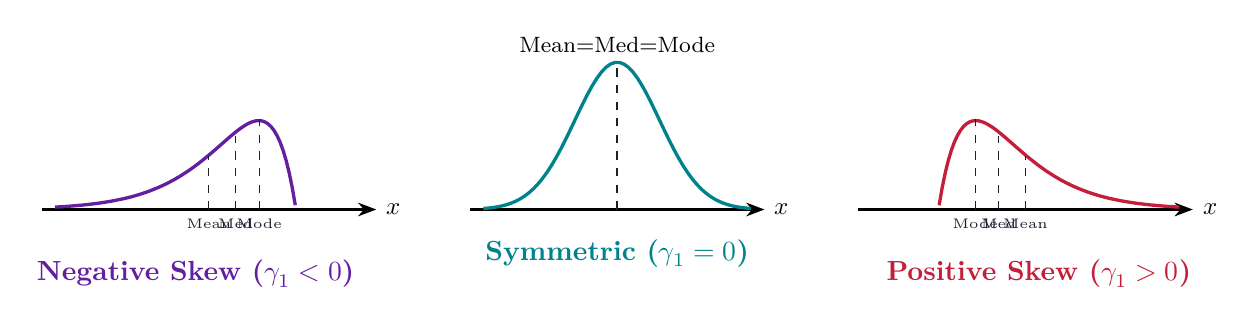
\begin{tikzpicture}[scale=0.85, every node/.style={font=\small}]
  % Symmetrical (Center)
  \begin{scope}[shift={(0,0)}]
    \draw[-Stealth, thick] (-2.2,0) -- (2.2,0) node[right] {$x$};
    \draw[very thick, color=myteal, domain=-2:2, samples=60] plot (\x, {2.2*exp(-(\x)^2/0.8)});
    \draw[dashed, thick, color=mydark] (0,0) -- (0,2.2);
    \node[above, font=\footnotesize] at (0,2.2) {Mean=Med=Mode};
    \node[below, font=\bfseries, color=myteal] at (0,-0.3) {Symmetric ($\gamma_1 = 0$)};
  \end{scope}

  % Positively Skewed (Right)
  \begin{scope}[shift={(4.8,0)}]
    \draw[-Stealth, thick] (-1.2,0) -- (3.8,0) node[right] {$x$};
    \draw[very thick, color=myred, domain=0.01:3.6, samples=80] plot (\x, {6.5*\x*exp(-1.8*\x)});
    \draw[dashed, thin, color=mydark] (0.55,0) node[below, font=\tiny] {Mode} -- (0.55,1.35);
    \draw[dashed, thin, color=mydark] (0.9,0) node[below, font=\tiny] {Med} -- (0.9,1.1);
    \draw[dashed, thin, color=mydark] (1.3,0) node[below, font=\tiny] {Mean} -- (1.3,0.8);
    \node[below, font=\bfseries, color=myred] at (1.5,-0.6) {Positive Skew ($\gamma_1 > 0$)};
  \end{scope}

  % Negatively Skewed (Left)
  \begin{scope}[shift={(-4.8,0)}]
    \draw[-Stealth, thick] (-3.8,0) -- (1.2,0) node[right] {$x$};
    \draw[very thick, color=mypurple, domain=-3.6:-0.01, samples=80] plot (\x, {-6.5*\x*exp(1.8*\x)});
    \draw[dashed, thin, color=mydark] (-1.3,0) node[below, font=\tiny] {Mean} -- (-1.3,0.8);
    \draw[dashed, thin, color=mydark] (-0.9,0) node[below, font=\tiny] {Med} -- (-0.9,1.1);
    \draw[dashed, thin, color=mydark] (-0.55,0) node[below, font=\tiny] {Mode} -- (-0.55,1.35);
    \node[below, font=\bfseries, color=mypurple] at (-1.5,-0.6) {Negative Skew ($\gamma_1 < 0$)};
  \end{scope}
\end{tikzpicture}
\end{center}
\end{tcolorbox}

\subsection{Measures of Kurtosis (Peakedness)}
\begin{tcolorbox}[defbox, title={\textbf{Definition: Kurtosis Coefficients $\beta_2$ and $\gamma_2$}}]
Kurtosis quantifies the degree of peakedness and the heaviness of the tails of a frequency curve relative to the standard normal bell curve:
\begin{equation}
  \beta_2 = \frac{\mu_4}{\mu_2^2} = \frac{\mu_4}{\sigma^4}, \qquad \gamma_2 = \beta_2 - 3
\end{equation}
\begin{itemize}[leftmargin=*, itemsep=2pt]
  \item \textbf{Mesokurtic ($\beta_2 = 3, \gamma_2 = 0$):} Normal distribution curve profile.
  \item \textbf{Leptokurtic ($\beta_2 > 3, \gamma_2 > 0$):} Sharply peaked center with heavy, fat tails (e.g., Student's $t$, Laplace).
  \item \textbf{Platykurtic ($\beta_2 < 3, \gamma_2 < 0$):} Flatter plateau-like peak with light, rapidly vanishing tails (e.g., Uniform distribution where $\beta_2 = 1.8$).
\end{itemize}
\end{tcolorbox}

% ───────────────────────────────────────────────────────────────────────────────
\section{Evaluation of Statistical Parameters for Core Distributions}
% ───────────────────────────────────────────────────────────────────────────────

\subsection{Binomial Distribution: Parameters and Recurrence Relation}
For $X \sim \text{Bin}(n, p)$ with $q = 1-p$:
\begin{equation}
  M_X(t) = \sum_{k=0}^n e^{tk} \binom{n}{k} p^k q^{n-k} = (q + p e^t)^n
\end{equation}
\begin{align}
  E[X] &= \mu = np, \qquad \operatorname{Var}(X) = \sigma^2 = npq \\[3pt]
  \mu_3 &= npq(q - p), \qquad \mu_4 = 3n^2 p^2 q^2 + npq(1 - 6pq) \\[3pt]
  \beta_1 &= \frac{\mu_3^2}{\mu_2^3} = \frac{(q-p)^2}{npq}, \qquad \beta_2 = \frac{\mu_4}{\mu_2^2} = 3 + \frac{1 - 6pq}{npq}
\end{align}
\textit{Recurrence Relation for Central Moments:}
\begin{equation}
  \mu_{r+1} = pq \left[n r \mu_{r-1} + \frac{d\mu_r}{dp}\right]
\end{equation}

\subsection{Poisson Distribution: Parameters and Recurrence Relation}
For $X \sim \text{Poisson}(\lambda)$:
\begin{equation}
  M_X(t) = \sum_{k=0}^\infty e^{tk} \frac{\lambda^k e^{-\lambda}}{k!} = e^{-\lambda} \sum_{k=0}^\infty \frac{(\lambda e^t)^k}{k!} = e^{-\lambda} e^{\lambda e^t} = \exp\left(\lambda(e^t - 1)\right)
\end{equation}
\begin{align}
  E[X] &= \lambda, \qquad \operatorname{Var}(X) = \lambda \\[3pt]
  \mu_3 &= \lambda, \qquad \mu_4 = 3\lambda^2 + \lambda \\[3pt]
  \beta_1 &= \frac{\mu_3^2}{\mu_2^3} = \frac{\lambda^2}{\lambda^3} = \frac{1}{\lambda}, \qquad \beta_2 = \frac{3\lambda^2 + \lambda}{\lambda^2} = 3 + \frac{1}{\lambda}
\end{align}
\textit{Recurrence Relation for Central Moments:}
\begin{equation}
  \mu_{r+1} = \lambda \left[r \mu_{r-1} + \frac{d\mu_r}{d\lambda}\right]
\end{equation}
As $\lambda \to \infty$, both $\beta_1 \to 0$ and $\beta_2 \to 3$, confirming convergence of Poisson to Normal!

\subsection{Normal Distribution: Parameters and Recurrence Relation}
For $X \sim \mathcal{N}(\mu, \sigma^2)$:
\begin{align}
  E[X] &= \mu, \qquad \operatorname{Var}(X) = \sigma^2 \\[3pt]
  \mu_{2k+1} &= 0 \quad \forall k \in \mathbb{N}_0, \qquad \mu_{2k} = \frac{(2k)!}{2^k k!} \sigma^{2k} \\[3pt]
  \beta_1 &= 0, \qquad \beta_2 = \frac{3\sigma^4}{\sigma^4} = 3 \iff \gamma_2 = 0
\end{align}
\textit{Recurrence Relation for Even Central Moments:}
\begin{equation}
  \mu_{2k} = (2k - 1) \sigma^2 \mu_{2k-2}
\end{equation}

% ───────────────────────────────────────────────────────────────────────────────
\section{Correlation and Regression Analysis}
% ───────────────────────────────────────────────────────────────────────────────

\subsection{Karl Pearson's Coefficient of Correlation ($r$)}
Karl Pearson's product-moment correlation coefficient $r$ provides a scale-invariant measure of linear association between two paired variables $(x_i, y_i)$:
\begin{tcolorbox}[formulabox, title={\textbf{Formula for Pearson's Correlation Coefficient}}]
\begin{equation}
  r = \frac{\operatorname{Cov}(X, Y)}{\sigma_x \sigma_y} = \frac{\displaystyle\sum_{i=1}^n (x_i - \bar{x})(y_i - \bar{y})}{\sqrt{\displaystyle\sum_{i=1}^n (x_i - \bar{x})^2} \sqrt{\displaystyle\sum_{i=1}^n (y_i - \bar{y})^2}} = \frac{n \sum x_i y_i - (\sum x_i)(\sum y_i)}{\sqrt{n\sum x_i^2 - (\sum x_i)^2}\sqrt{n\sum y_i^2 - (\sum y_i)^2}}
\end{equation}
\textbf{Properties of $r$:}
\begin{enumerate}[leftmargin=*, itemsep=2pt]
  \item Normalized limits: $-1 \le r \le +1$.
  \item Invariant to change of origin and scale: If $u = \frac{x - a}{h}$ and $v = \frac{y - b}{k}$ with $h, k > 0$, then $r_{xy} = r_{uv}$.
\end{enumerate}
\end{tcolorbox}

\subsection{Linear Regression Equations and Least Squares}
Regression expresses the average functional relationship predicting a dependent variable from an independent variable.
\begin{tcolorbox}[defbox, title={\textbf{The Two Lines of Regression}}]
\textbf{1. Line of Regression of $Y$ on $X$:} Predicts $Y$ for a known value of $X$:
\begin{equation}
  Y - \bar{y} = b_{yx} (X - \bar{x}), \qquad b_{yx} = r \frac{\sigma_y}{\sigma_x} = \frac{\operatorname{Cov}(X, Y)}{\sigma_x^2}
\end{equation}
\textbf{2. Line of Regression of $X$ on $Y$:} Predicts $X$ for a known value of $Y$:
\begin{equation}
  X - \bar{x} = b_{xy} (Y - \bar{y}), \qquad b_{xy} = r \frac{\sigma_x}{\sigma_y} = \frac{\operatorname{Cov}(X, Y)}{\sigma_y^2}
\end{equation}
where $b_{yx}$ and $b_{xy}$ are the \textbf{regression coefficients}.
\end{tcolorbox}

\begin{tcolorbox}[formulabox, title={\textbf{Key Properties of Regression Coefficients}}]
\begin{enumerate}[leftmargin=*, itemsep=3pt]
  \item \textbf{Geometric Mean Property:} The correlation coefficient is the geometric mean of the regression coefficients:
  \begin{equation}
    r = \pm \sqrt{b_{yx} \cdot b_{xy}}
  \end{equation}
  Both regression coefficients must share the same algebraic sign, which is also the sign of $r$.
  \item \textbf{Reciprocal Magnitude Constraint:} If $b_{yx} > 1$, then $b_{xy} < 1$, since $b_{yx} b_{xy} = r^2 \le 1$.
  \item \textbf{Arithmetic Mean Inequality:} $\dfrac{b_{yx} + b_{xy}}{2} \ge r$ (by AM $\ge$ GM).
  \item \textbf{Centroid Intersection:} Both lines intersect at the point of means $(\bar{x}, \bar{y})$.
  \item \textbf{Scale Dependence:} Regression coefficients are invariant to change of origin, but \textbf{depend} on scale: $b_{yx} = \frac{k}{h} b_{vu}$.
\end{enumerate}
\end{tcolorbox}

\subsection{Angle Between the Two Regression Lines}
\begin{tcolorbox}[examplebox, title={\textbf{Derivation: Angle $\theta$ Between Regression Lines}}]
The slopes of the two lines in the $(X, Y)$ plane are:
\begin{equation}
  m_1 = b_{yx} = r \frac{\sigma_y}{\sigma_x}, \qquad m_2 = \frac{1}{b_{xy}} = \frac{\sigma_y}{r \sigma_x}
\end{equation}
The angle $\theta$ between the lines satisfies:
\begin{equation}
  \tan\theta = \left|\frac{m_2 - m_1}{1 + m_1 m_2}\right| = \left|\frac{\frac{\sigma_y}{r\sigma_x} - r\frac{\sigma_y}{\sigma_x}}{1 + \left(r\frac{\sigma_y}{\sigma_x}\right)\left(\frac{\sigma_y}{r\sigma_x}\right)}\right| = \left|\frac{\frac{\sigma_y}{\sigma_x}\left(\frac{1 - r^2}{r}\right)}{1 + \frac{\sigma_y^2}{\sigma_x^2}}\right|
\end{equation}
Simplifying the denominator $1 + \sigma_y^2/\sigma_x^2 = (\sigma_x^2 + \sigma_y^2)/\sigma_x^2$:
\begin{equation}
  \tan\theta = \left(\frac{1 - r^2}{|r|}\right) \left(\frac{\sigma_x \sigma_y}{\sigma_x^2 + \sigma_y^2}\right)
\end{equation}
\textbf{Special Cases:}
\begin{itemize}[leftmargin=*, itemsep=2pt]
  \item If $r = \pm 1 \implies \tan\theta = 0 \implies \theta = 0^\circ$ (the two lines \textbf{coincide}; perfect linear correlation).
  \item If $r = 0 \implies \tan\theta \to \infty \implies \theta = 90^\circ$ (the two lines are \textbf{perpendicular} parallel to coordinate axes; uncorrelated).
\end{itemize}
\end{tcolorbox}

\begin{tcolorbox}[tikzbox, title={\textbf{TikZ Plot: Scatter Diagram and the Two Lines of Regression with Intersection at Centroid}}]
\begin{center}
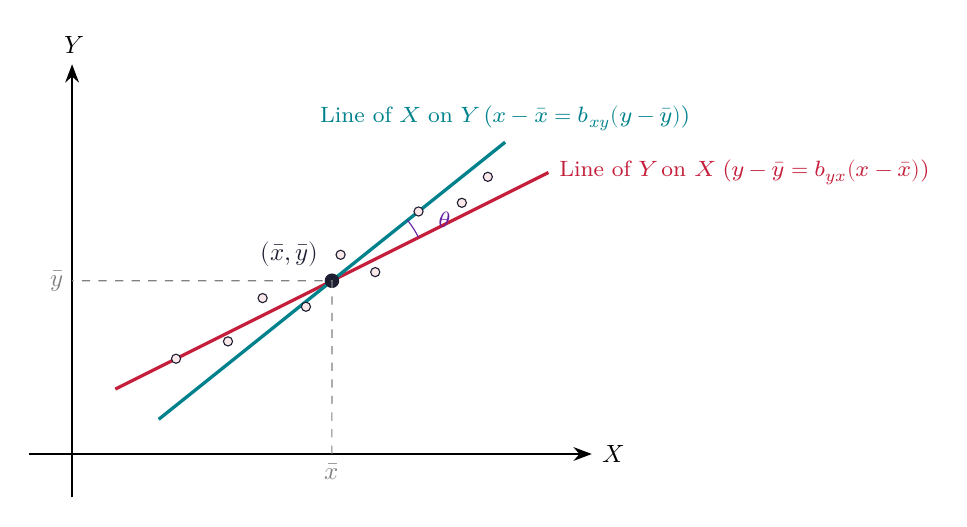
\begin{tikzpicture}[scale=1.1, every node/.style={font=\small}]
  % Axes
  \draw[-Stealth, thick] (-0.5, 0) -- (6.0, 0) node[right] {$X$};
  \draw[-Stealth, thick] (0, -0.5) -- (0, 4.5) node[above] {$Y$};

  % Centroid point (x_bar, y_bar) = (3, 2)
  \coordinate (C) at (3.0, 2.0);

  % Line of Y on X: y - 2 = 0.5(x - 3) -> slope 0.5
  \draw[very thick, color=myred] (0.5, 0.75) -- (5.5, 3.25)
    node[right, font=\footnotesize] {Line of $Y$ on $X$ ($y - \bar{y} = b_{yx}(x - \bar{x})$)};

  % Line of X on Y: x - 3 = 1.25(y - 2) -> y - 2 = 0.8(x - 3) -> slope 0.8
  \draw[very thick, color=myteal] (1.0, 0.4) -- (5.0, 3.6)
    node[above, font=\footnotesize] {Line of $X$ on $Y$ ($x - \bar{x} = b_{xy}(y - \bar{y})$)};

  % Centroid marker
  \filldraw[color=mydark] (C) circle (2.2pt) node[above left=2pt] {$(\bar{x}, \bar{y})$};
  \draw[dashed, thin, color=gray] (3.0, 0) node[below] {$\bar{x}$} -- (C) -- (0, 2.0) node[left] {$\bar{y}$};

  % Angle arc between lines
  \draw[thin, color=mypurple] (4.0, 2.5) arc (26.5:38.6:1.12);
  \node[color=mypurple, font=\footnotesize] at (4.3, 2.7) {$\theta$};

  % Scatter sample points
  \foreach \p in {(1.2, 1.1), (1.8, 1.3), (2.2, 1.8), (2.7, 1.7), (3.1, 2.3), (3.5, 2.1), (4.0, 2.8), (4.5, 2.9), (4.8, 3.2)} {
    \filldraw[color=mydark, fill=hdrred] \p circle (1.5pt);
  }
\end{tikzpicture}
\end{center}
\end{tcolorbox}

\subsection{Spearman's Rank Correlation Coefficient ($r_s$)}
When variables represent qualitative attributes that cannot be measured numerically but can be ordered or ranked (e.g., beauty, intelligence, performance rankings):
\begin{tcolorbox}[defbox, title={\textbf{Spearman's Rank Correlation Formula}}]
Let $R_{xi}$ and $R_{yi}$ denote the ranks assigned to the $i$-th individual, with difference $d_i = R_{xi} - R_{yi}$.
\begin{enumerate}[leftmargin=*, itemsep=3pt]
  \item \textbf{Case 1: When Ranks are Distinct (No Ties):}
  \begin{equation}
    r_s = 1 - \frac{6 \displaystyle\sum_{i=1}^n d_i^2}{n(n^2 - 1)}
  \end{equation}
  \item \textbf{Case 2: When Ranks are Tied (Correction Factor):} If an attribute value repeats $m$ times, all tied entries are allocated the average rank, and a correction factor $\frac{m(m^2 - 1)}{12}$ is added for each tie group:
  \begin{equation}
    r_s = 1 - \frac{6 \left[\displaystyle\sum_{i=1}^n d_i^2 + \sum_{j} \frac{m_j(m_j^2 - 1)}{12}\right]}{n(n^2 - 1)}
  \end{equation}
\end{enumerate}
\end{tcolorbox}

\newpage
% ===============================================================================
% MANDATORY QUICK REVISION PAGE
% ===============================================================================
\begin{center}
  {\large\bfseries\color{myred} Quick Revision --- Module 4}\\[1pt]
  {\small\color{mydark} Basic Statistics, Moments, Distributions, Correlation and Regression $|$ BS-M301}
\end{center}
\noindent{\color{myred}\rule{\linewidth}{1.0pt}}
\vspace{1pt}

\begin{tcolorbox}[formulabox, top=2pt, bottom=2pt, title={\textbf{Key Formulas and Statistical Identities at a Glance}}]
\renewcommand{\arraystretch}{0.96}
\setlength{\tabcolsep}{3.5pt}
\begin{tabularx}{\linewidth}{B{3.8cm} X}
Empirical Mean-Mode & $\text{Mode} \approx 3\text{Median} - 2\text{Mean} \iff \text{Mean}-\text{Mode} \approx 3(\text{Mean}-\text{Median})$ \\[0.2pt]
Central from Raw Moments & $\mu_2 = \mu_2'-(\mu_1')^2, \; \mu_3 = \mu_3'-3\mu_2'\mu_1'+2(\mu_1')^3, \; \mu_4 = \mu_4'-4\mu_3'\mu_1'+6\mu_2'(\mu_1')^2-3(\mu_1')^4$ \\[0.2pt]
Pearson Skewness & $S_k = \frac{\text{Mean}-\text{Mode}}{\sigma} = \frac{3(\text{Mean}-\text{Median})}{\sigma}, \quad \beta_1 = \frac{\mu_3^2}{\mu_2^3}, \quad \gamma_1 = \frac{\mu_3}{\sigma^3}$ \\[0.2pt]
Kurtosis Coefficients & $\beta_2 = \frac{\mu_4}{\mu_2^2} = \frac{\mu_4}{\sigma^4}, \quad \gamma_2 = \beta_2 - 3 \quad (\text{Meso}=3, \text{Lepto}>3, \text{Platy}<3)$ \\[0.2pt]
Binomial Parameters & $\mu = np, \quad \sigma^2 = npq, \quad \beta_1 = \frac{(q-p)^2}{npq}, \quad \beta_2 = 3 + \frac{1-6pq}{npq}$ \\[0.2pt]
Poisson Parameters & $\mu = \lambda, \quad \sigma^2 = \lambda, \quad \beta_1 = \frac{1}{\lambda}, \quad \beta_2 = 3 + \frac{1}{\lambda}$ \\[0.2pt]
Normal Moments & All odd $\mu_{2k+1}=0, \quad \mu_{2k} = \frac{(2k)!}{2^k k!} \sigma^{2k}, \quad \beta_1 = 0, \quad \beta_2 = 3$ \\[0.2pt]
Pearson Correlation & $r = \frac{\operatorname{Cov}(X,Y)}{\sigma_x \sigma_y} = \frac{\sum(x-\bar{x})(y-\bar{y})}{\sqrt{\sum(x-\bar{x})^2\sum(y-\bar{y})^2}} \in [-1, +1]$ \\[0.2pt]
Regression Lines & $Y-\bar{y} = b_{yx}(X-\bar{x}), \quad X-\bar{x} = b_{xy}(Y-\bar{y}), \quad b_{yx} = r\frac{\sigma_y}{\sigma_x}, \; b_{xy} = r\frac{\sigma_x}{\sigma_y}$ \\[0.2pt]
Regression Properties & $r = \pm\sqrt{b_{yx} b_{xy}}, \quad \frac{b_{yx}+b_{xy}}{2} \ge r, \quad \tan\theta = \frac{1-r^2}{|r|}\frac{\sigma_x \sigma_y}{\sigma_x^2+\sigma_y^2}$ \\[0.2pt]
Spearman Rank Corr. & $r_s = 1 - \frac{6\sum d_i^2}{n(n^2-1)} \quad (\text{Ties add } \sum\frac{m_j(m_j^2-1)}{12})$ \\
\end{tabularx}
\end{tcolorbox}

\vspace{1pt}

\begin{tcolorbox}[defbox, top=2pt, bottom=2pt, title={\textbf{One-Line Definitions}}]
\begin{itemize}[leftmargin=*, itemsep=-0.5pt, topsep=0pt, parsep=0pt]
  \item \textbf{Arithmetic Mean:} Center of gravity of data where algebraic sum of deviations $\sum(x_i - \bar{x})$ is identically zero.
  \item \textbf{Median \& Mode:} Median is positional 50th percentile; Mode is observation exhibiting peak frequency density.
  \item \textbf{Skewness:} Metric quantifying directional asymmetry of frequency curve tail relative to central peak.
  \item \textbf{Kurtosis:} Measure of peakedness and tail fatness relative to standard Gaussian benchmark ($\beta_2 = 3$).
  \item \textbf{Leptokurtic Curve:} Sharply peaked frequency profile with fat heavy tails exhibiting $\beta_2 > 3$.
  \item \textbf{Platykurtic Curve:} Broad-shouldered flattened frequency curve with light rapidly decaying tails ($\beta_2 < 3$).
  \item \textbf{Pearson's $r$:} Standardized dimensionless measure of the strength and direction of linear association.
  \item \textbf{Regression Line:} Optimal line minimizing sum of squared vertical/horizontal prediction errors (Least Squares).
  \item \textbf{Regression Coefficients:} Directional slopes $b_{yx}$ and $b_{xy}$ whose geometric mean equals correlation coefficient $r$.
  \item \textbf{Spearman's Rank Correlation:} Non-parametric correlation measuring monotonic agreement between ordinal rankings.
\end{itemize}
\end{tcolorbox}

\newpage

\begin{tcolorbox}[exambox, title={\textbf{Frequently Asked / Viva Questions (Part 1)}}]
\begin{enumerate}[topsep=0pt, label=\textbf{Q\arabic*.}, itemsep=3.2pt]
  \item \Q{State the algebraic properties of the Arithmetic Mean.}
  (1) The sum of deviations of all observations from their arithmetic mean is zero: $\sum f_i (x_i - \bar{x}) = 0$. (2) The sum of squared deviations is minimal when taken about the mean: $\sum f_i (x_i - A)^2$ is minimum for $A = \bar{x}$. (3) Mean of combined series: $\bar{x}_{12} = \frac{n_1 \bar{x}_1 + n_2 \bar{x}_2}{n_1 + n_2}$.

  \item \Q{Derive the relationship $\mu_3 = \mu_3' - 3\mu_2'\mu_1' + 2(\mu_1')^3$.}
  $\mu_3 = E[(X - \mu)^3] = E[X^3 - 3X^2\mu + 3X\mu^2 - \mu^3] = E[X^3] - 3\mu E[X^2] + 3\mu^2 E[X] - \mu^3$. Substituting $E[X] = \mu_1', E[X^2] = \mu_2', E[X^3] = \mu_3'$: $\mu_3 = \mu_3' - 3\mu_1'\mu_2' + 3(\mu_1')^3 - (\mu_1')^3 = \mu_3' - 3\mu_2'\mu_1' + 2(\mu_1')^3$.

  \item \Q{Distinguish between positive skewness and negative skewness with sketches.}
  In positive skewness, the tail is extended to the right, and $\text{Mean} > \text{Median} > \text{Mode}$ ($\gamma_1 > 0$). In negative skewness, the tail is extended to the left, and $\text{Mode} > \text{Median} > \text{Mean}$ ($\gamma_1 < 0$).

  \item \Q{What are Leptokurtic, Mesokurtic and Platykurtic curves?}
  A curve with $\beta_2 = 3$ is Mesokurtic (Normal). If $\beta_2 > 3$, it is Leptokurtic (more peaked with heavier tails). If $\beta_2 < 3$, it is Platykurtic (flatter top with lighter tails).

  \item \Q{State the recurrence relation for central moments of a Poisson distribution.}
  $\mu_{r+1} = \lambda \left[r \mu_{r-1} + \frac{d\mu_r}{d\lambda}\right]$. For $r=1$: $\mu_2 = \lambda(1\cdot 0 + 1) = \lambda$. For $r=2$: $\mu_3 = \lambda(2\cdot 0 + \frac{d\lambda}{d\lambda}) = \lambda$. For $r=3$: $\mu_4 = \lambda(3\lambda + \frac{d\lambda}{d\lambda}) = 3\lambda^2 + \lambda$.

  \item \Q{Prove that the correlation coefficient is the geometric mean of the two regression coefficients.}
  $b_{yx} = r \frac{\sigma_y}{\sigma_x}$ and $b_{xy} = r \frac{\sigma_x}{\sigma_y}$. Multiplying: $b_{yx} \cdot b_{xy} = \left(r\frac{\sigma_y}{\sigma_x}\right)\left(r\frac{\sigma_x}{\sigma_y}\right) = r^2$. Taking the square root: $r = \pm \sqrt{b_{yx} \cdot b_{xy}}$.

  \item \Q{Can two regression coefficients be $1.5$ and $0.8$? Explain.}
  Yes! $b_{yx} \cdot b_{xy} = (1.5)(0.8) = 1.2 > 1$. But wait: $r^2 = b_{yx} b_{xy} \le 1$. Since $1.2 > 1$, this would imply $r^2 > 1$, which violates the Cauchy-Schwarz bound $|r| \le 1$. Hence $b_{yx}=1.5$ and $b_{xy}=0.8$ is impossible!
\end{enumerate}
\end{tcolorbox}

\newpage

\begin{tcolorbox}[exambox, top=3pt, bottom=3pt, title={\textbf{Frequently Asked / Viva Questions (Part 2)}}]
\begin{enumerate}[topsep=0pt, label=\textbf{Q\arabic*.}, itemsep=1.8pt, start=8]
  \item \Q{Why are there two lines of regression rather than a single line?}
  Because the regression of $Y$ on $X$ minimizes the sum of squared vertical errors $\sum (y_i - \hat{y}_i)^2$, whereas the regression of $X$ on $Y$ minimizes the sum of squared horizontal errors $\sum (x_i - \hat{x}_i)^2$. The two lines coincide if and only if $r = \pm 1$ (zero error).

  \item \Q{State the formula for the angle $\theta$ between the two regression lines and interpret the extreme cases.}
  $\tan\theta = \frac{1-r^2}{|r|}\frac{\sigma_x \sigma_y}{\sigma_x^2 + \sigma_y^2}$. If $r = \pm 1$, $\tan\theta = 0 \implies \theta = 0^\circ$ (lines coincide; perfect correlation). If $r = 0$, $\tan\theta = \infty \implies \theta = 90^\circ$ (lines are perpendicular; uncorrelated).

  \item \Q{Derive Spearman's Rank Correlation formula when ranks are not tied.}
  Let $x_i, y_i$ be ranks from $1$ to $n$. Then $\bar{x} = \bar{y} = \frac{n+1}{2}$, $\sigma_x^2 = \sigma_y^2 = \frac{n^2-1}{12}$. Since $d_i = x_i - y_i$, $\sum d_i^2 = \sum (x_i - \bar{x})^2 + \sum (y_i - \bar{y})^2 - 2\sum (x_i - \bar{x})(y_i - \bar{y}) = 2n\sigma_x^2 - 2n r \sigma_x^2 = 2n\sigma_x^2(1 - r_s)$. Substituting $\sigma_x^2 = \frac{n^2-1}{12}$ yields $r_s = 1 - \frac{6\sum d_i^2}{n(n^2-1)}$.
\end{enumerate}
\end{tcolorbox}

\vspace{2pt}

\begin{tcolorbox}[tikzbox, top=3pt, bottom=3pt, title={\textbf{Summary Matrix: Comparison of Binomial, Poisson and Normal Distributions}}]
\par\vspace{1pt}\noindent
\begingroup
\setlength{\tabcolsep}{3.5pt}
\setlength{\extrarowheight}{1.0pt}
\renewcommand{\arraystretch}{1.12}
\begin{tabularx}{\linewidth}{|B{2.5cm}|B{3.2cm}|B{2.2cm}|B{2.5cm}|Y|}
\hline
\textbf{Parameter} & \textbf{Binomial $\text{Bin}(n, p)$} & \textbf{Poisson $\text{Poisson}(\lambda)$} & \textbf{Normal $\mathcal{N}(\mu, \sigma^2)$} & \textbf{Comparative Property} \\
\hline
Mean ($E[X]$) & $np$ & $\lambda$ & $\mu$ & Location measure. \\
\hline
Variance ($\sigma^2$) & $npq < \mu$ & $\lambda = \mu$ & $\sigma^2$ (Independent of $\mu$) & $\text{Var}_{\text{Bin}} < \text{Mean}$; $\text{Var}_{\text{Poi}} = \text{Mean}$. \\
\hline
MGF ($M_X(t)$) & $(q + p e^t)^n$ & $\exp(\lambda(e^t - 1))$ & $\exp(\mu t + \frac{1}{2}\sigma^2 t^2)$ & Poisson is limiting Binomial MGF. \\
\hline
Skewness ($\gamma_1$) & $\frac{q - p}{\sqrt{npq}}$ & $\frac{1}{\sqrt{\lambda}}$ & $0$ & Binomial is symmetric if $p = 0.5$. \\
\hline
Kurtosis ($\beta_2$) & $3 + \frac{1 - 6pq}{npq}$ & $3 + \frac{1}{\lambda}$ & $3$ ($\gamma_2 = 0$) & Both converge to $3$ as $n, \lambda \to \infty$. \\
\hline
\end{tabularx}
\endgroup
\end{tcolorbox}

\end{document}
